\subsubsection{Chiss}
\begin{samepage}
	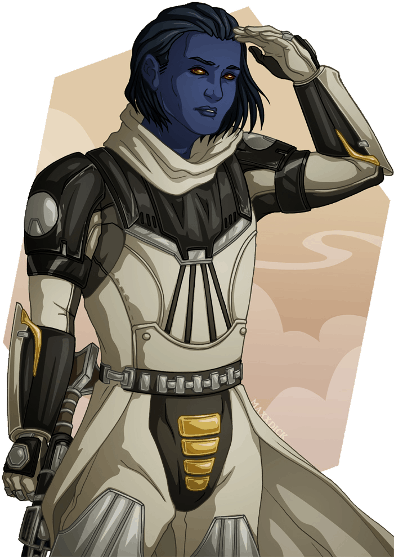
\includegraphics[width=5cm]{img/personnages/races/chiss.png}

	\vspace{-9\baselineskip}

	\begin{flushright}
		\begin{tabular}{ l l }
			\textbf{Type} 			& Humanoïde \\
		   	\textbf{Planète} 		& Csilla \\
		   	\textbf{Language} 		& Cheunh \\
		   	\textbf{Orientation} 	& Obscur \\
		\end{tabular}
	\end{flushright}
	\vspace{4\baselineskip}
\end{samepage}

Les Chiss font en moyenne 1,80m et ont une morphologie humaine. Cependant, il est impossible de les confondre à cause de leur peau bleue et de leurs yeux d’un rouge éclatant. Ils ont toujours des cheveux noirs, bien qu’avec les années, certains voient des cheveux blancs apparaitre. \\ 

La société Chiss est très évoluée. Ils ont de l’intérêt pour les arts et la science et maintiennent une puissante force militaire. Ils ont la réputation d’être de fins stratèges militaires mais leur façon de penser se retrouve dans tous les domaines de la vie quotidienne. Ils réfléchissent et pensent à différents points de vue et aux alternatives lorsqu’ils doivent prendre une décision.  

\begin{description}[align=left]
\item [Charismatique] 			% CAP +2 +2 +1
		Les Chiss sont des êtres charismatique habitué à commander des armées.\\
		\emph{+2 Cha}\\
		\emph{Commandement}\\
		\emph{d6 Connaissance (Combats)}
\item [Aquité visuelle] 		% CAP +1
		Les modifications qu’ont subies leurs yeux leur ont également donné une plus grande acuité visuelle.\\
		\emph{d6 Perception}
\item [Arrogant] 				% CAP -2
		Les Chiss sont fréquemment perçus par le reste de la galaxie, comme un peuple arrogant, calculateur et distant.\\
		\emph{Arrogant}
\item [Insensible à la Force] 		% CAP -1
		Les Chiss ne sont pas connus pour être une espèce sensible à la Force. Ils n’ont eut qu’un seul exemple d’individu sensible, en la personne de Sev’rance Tann. Cette dernière avait optée pour le côté obscur.\\
		\emph{A la création, l'augmentation de l'\^Ame coute 2pt}
\end{description}